% !TeX program  = xelatex
% !TeX encoding = UTF-8
% !TeX root     = course-work.tex
\documentclass{mirea}

% !TeX program  = xelatex
% !TeX encoding = UTF-8
% !TeX root     = article1.tex

\usepackage{hyperref}
\hypersetup{pdftitle={ВКР на тему "<Разработка системы для поиска и возврата утерянных вещей">}, pdfauthor={В. С. Верхотуров}}

\usepackage{comment}

\usepackage{graphicx}

\usepackage{listings}
\usepackage{xcolor}
\lstset{basicstyle=\footnotesize, breaklines=true, numbers=left, captionpos=t, showstringspaces=false, commentstyle=\color{teal}, stringstyle=\color{red}, keywordstyle=\color{violet}}  % Настройки, применяемые ко всем листингам

% Создание введения или заключения
\newcommand{\supersection}[1]{
	\section*{#1}
	\phantomsection
	\addcontentsline{toc}{section}{#1}
}

\usepackage{caption}
\captionsetup[lstlisting]{justification=raggedright, singlelinecheck=false}

\usepackage{pdfpages}

\usepackage{microtype}

\usepackage{multirow}

\usepackage{array}
\usepackage{setspace}
\newcolumntype{x}[1]{>{\setstretch{0.8}\small\centering\arraybackslash\hspace{0pt}}m{#1}}
\newcolumntype{y}[1]{>{\centering\arraybackslash\hspace{0pt}}m{#1}}
\usepackage{longtable}

\usepackage{float}

%\usepackage{color,xesearch}
%\SearchList{make-red}{\textcolor{red}{#1}}{эффективность,эффективности,эффективностью,эффективностей,эффективностям,эффективностями,эффективностях,эффективный,эффективная,эффективное,инновационный,иновационная,иновационные,инновация,иновационных,надежность,оптимизация,качество}


\begin{document}
	
% 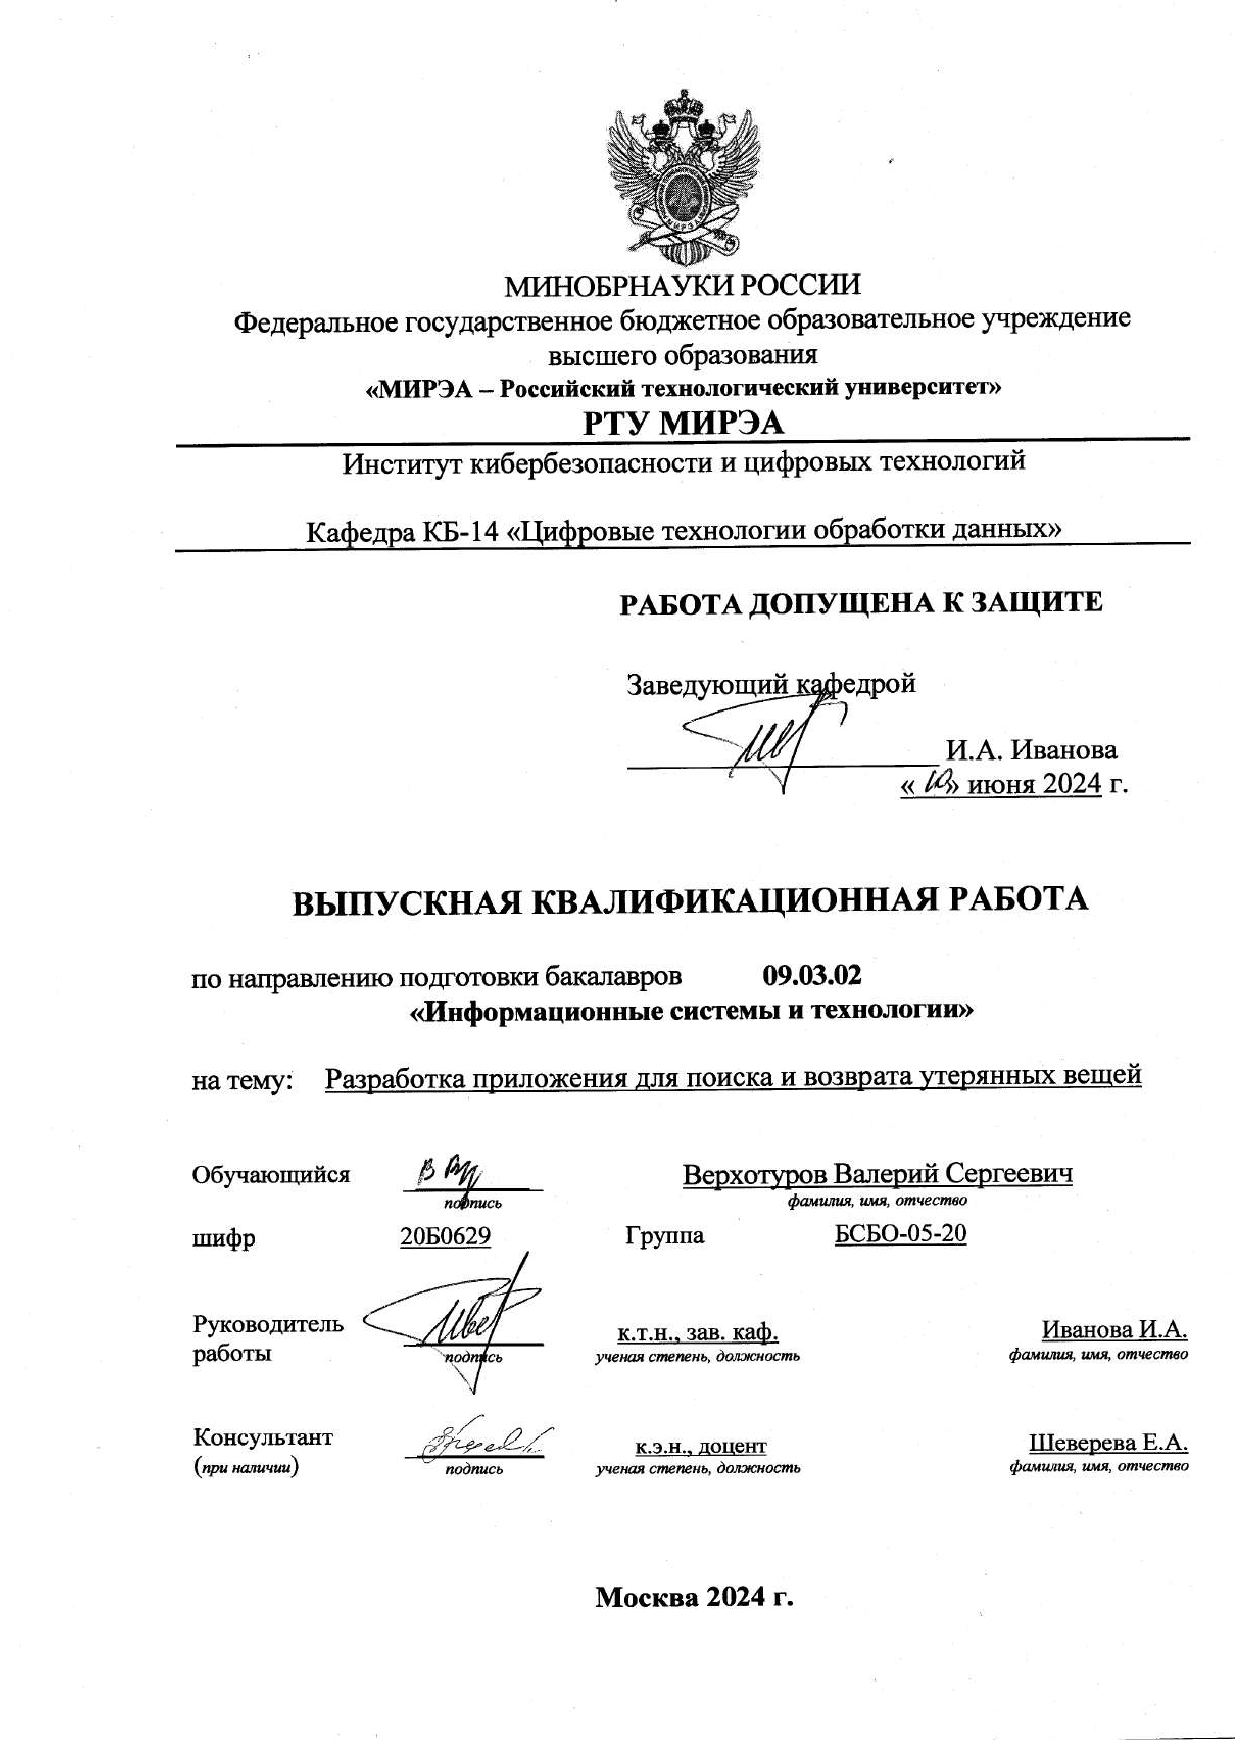
\includepdf[pages=-]{titlepage.pdf}
	
\addtocounter{page}{2}

% Содержание
\tableofcontents


\supersection{Введение}

Современный мир стал свидетелем стремительного развития информационных технологий, которые проникают во все сферы нашей жизни, включая поиск и нахождение утерянных вещей. В ситуации, когда мы потеряли что-то ценное или важное для нас, возникает огромная необходимость в удобном способе поиска и возврата утраченных предметов. Веб-сервис Бюро находок является одним из инновационных решений этой проблемы.

Целью данной курсовой работы является разработка и анализ веб-сер\-ви\-са Бюро находок, предоставляющего возможность пользователям объявлять о потерянных и найденных предметах, а также упрощающего процесс возврата утерянных вещей и связи между их владельцами и нашим сервисом.

Актуальность данного исследования обусловлена не только повседневными ситуациями потери вещей, но и ростом числа людей, пользующихся интернетом и смартфонами. Веб-сервис Бюро находок предлагает новый подход к организации процесса поиска и возврата утерянных предметов, обеспечивая удобство и оперативность взаимодействия между пользователями и нашим сервисом.

В аналитическом разделе будет проведен обзор существующих веб-сер\-ви\-сов и приложений, а также проанализированы их преимущества и недостатки. Специальный раздел посвящен разработке концепции Бюро находок, включая функциональные требования и особенности реализации. Технологический раздел описывает выбранные технологии и инструменты для разработки веб-сервиса. В экономическом разделе будет проведен расчет затрат на разработку и поддержку Бюро находок. В заключении будут подведены итоги работы и сделаны выводы о значимости и перспективах развития веб-сервиса Бюро находок.

Для написания данной курсовой работы будут использованы различные источники информации, включая научные статьи, публикации, книги и данные из сети Интернет. Все использованные источники будут тщательно приведены в списке использованных литературных источников в конце работы.

Цель данного исследования заключается в создании веб-сервиса Бюро находок, который поможет людям быстро и надежно находить утерянные вещи и обеспечит удобство взаимодействия с нашим сервисом. В дальнейшем этот веб-сервис может стать платформой для реализации дополнительных функций и услуг, связанных с восстановлением утерянных вещей и повышением безопасности собственности.


\section{Аналитический раздел}

В аналитическом разделе данной работы будет представлен полный обзор существующих веб-сервисов и приложений, которые функционируют в интернете. В рамках этого обзора будет проведен детальный анализ каждого из них, включая выявление и описание их преимуществ и недостатков. Такой подход позволит получить всестороннее представление о разнообразии веб-сервисов и приложений, а также сделать осведомленный выбор, учитывая их положительные и отрицательные аспекты. В результате данного анализа будут получены ценные выводы, которые помогут пользователям определиться с выбором наиболее подходящего веб-сервиса или приложения в соответствии с их потребностями и предпочтениями.

\subsection{Статистика потерянных и найденных вещей}

Статистика, взятая с сайта \href{http://xn--80aisbkedbuk1b.xn--p1ai/}{столнаходок.рф}, утверждает, что только 20\% пользователей их сайта смогли установить и вернуть вещи. Также на рисунках \ref{fig:chart2023} и \ref{fig:chart2022} представлена гистограмма количества созданных объявлений за 2022 и 2023 года.

\begin{figure}[htb]
	\centering
	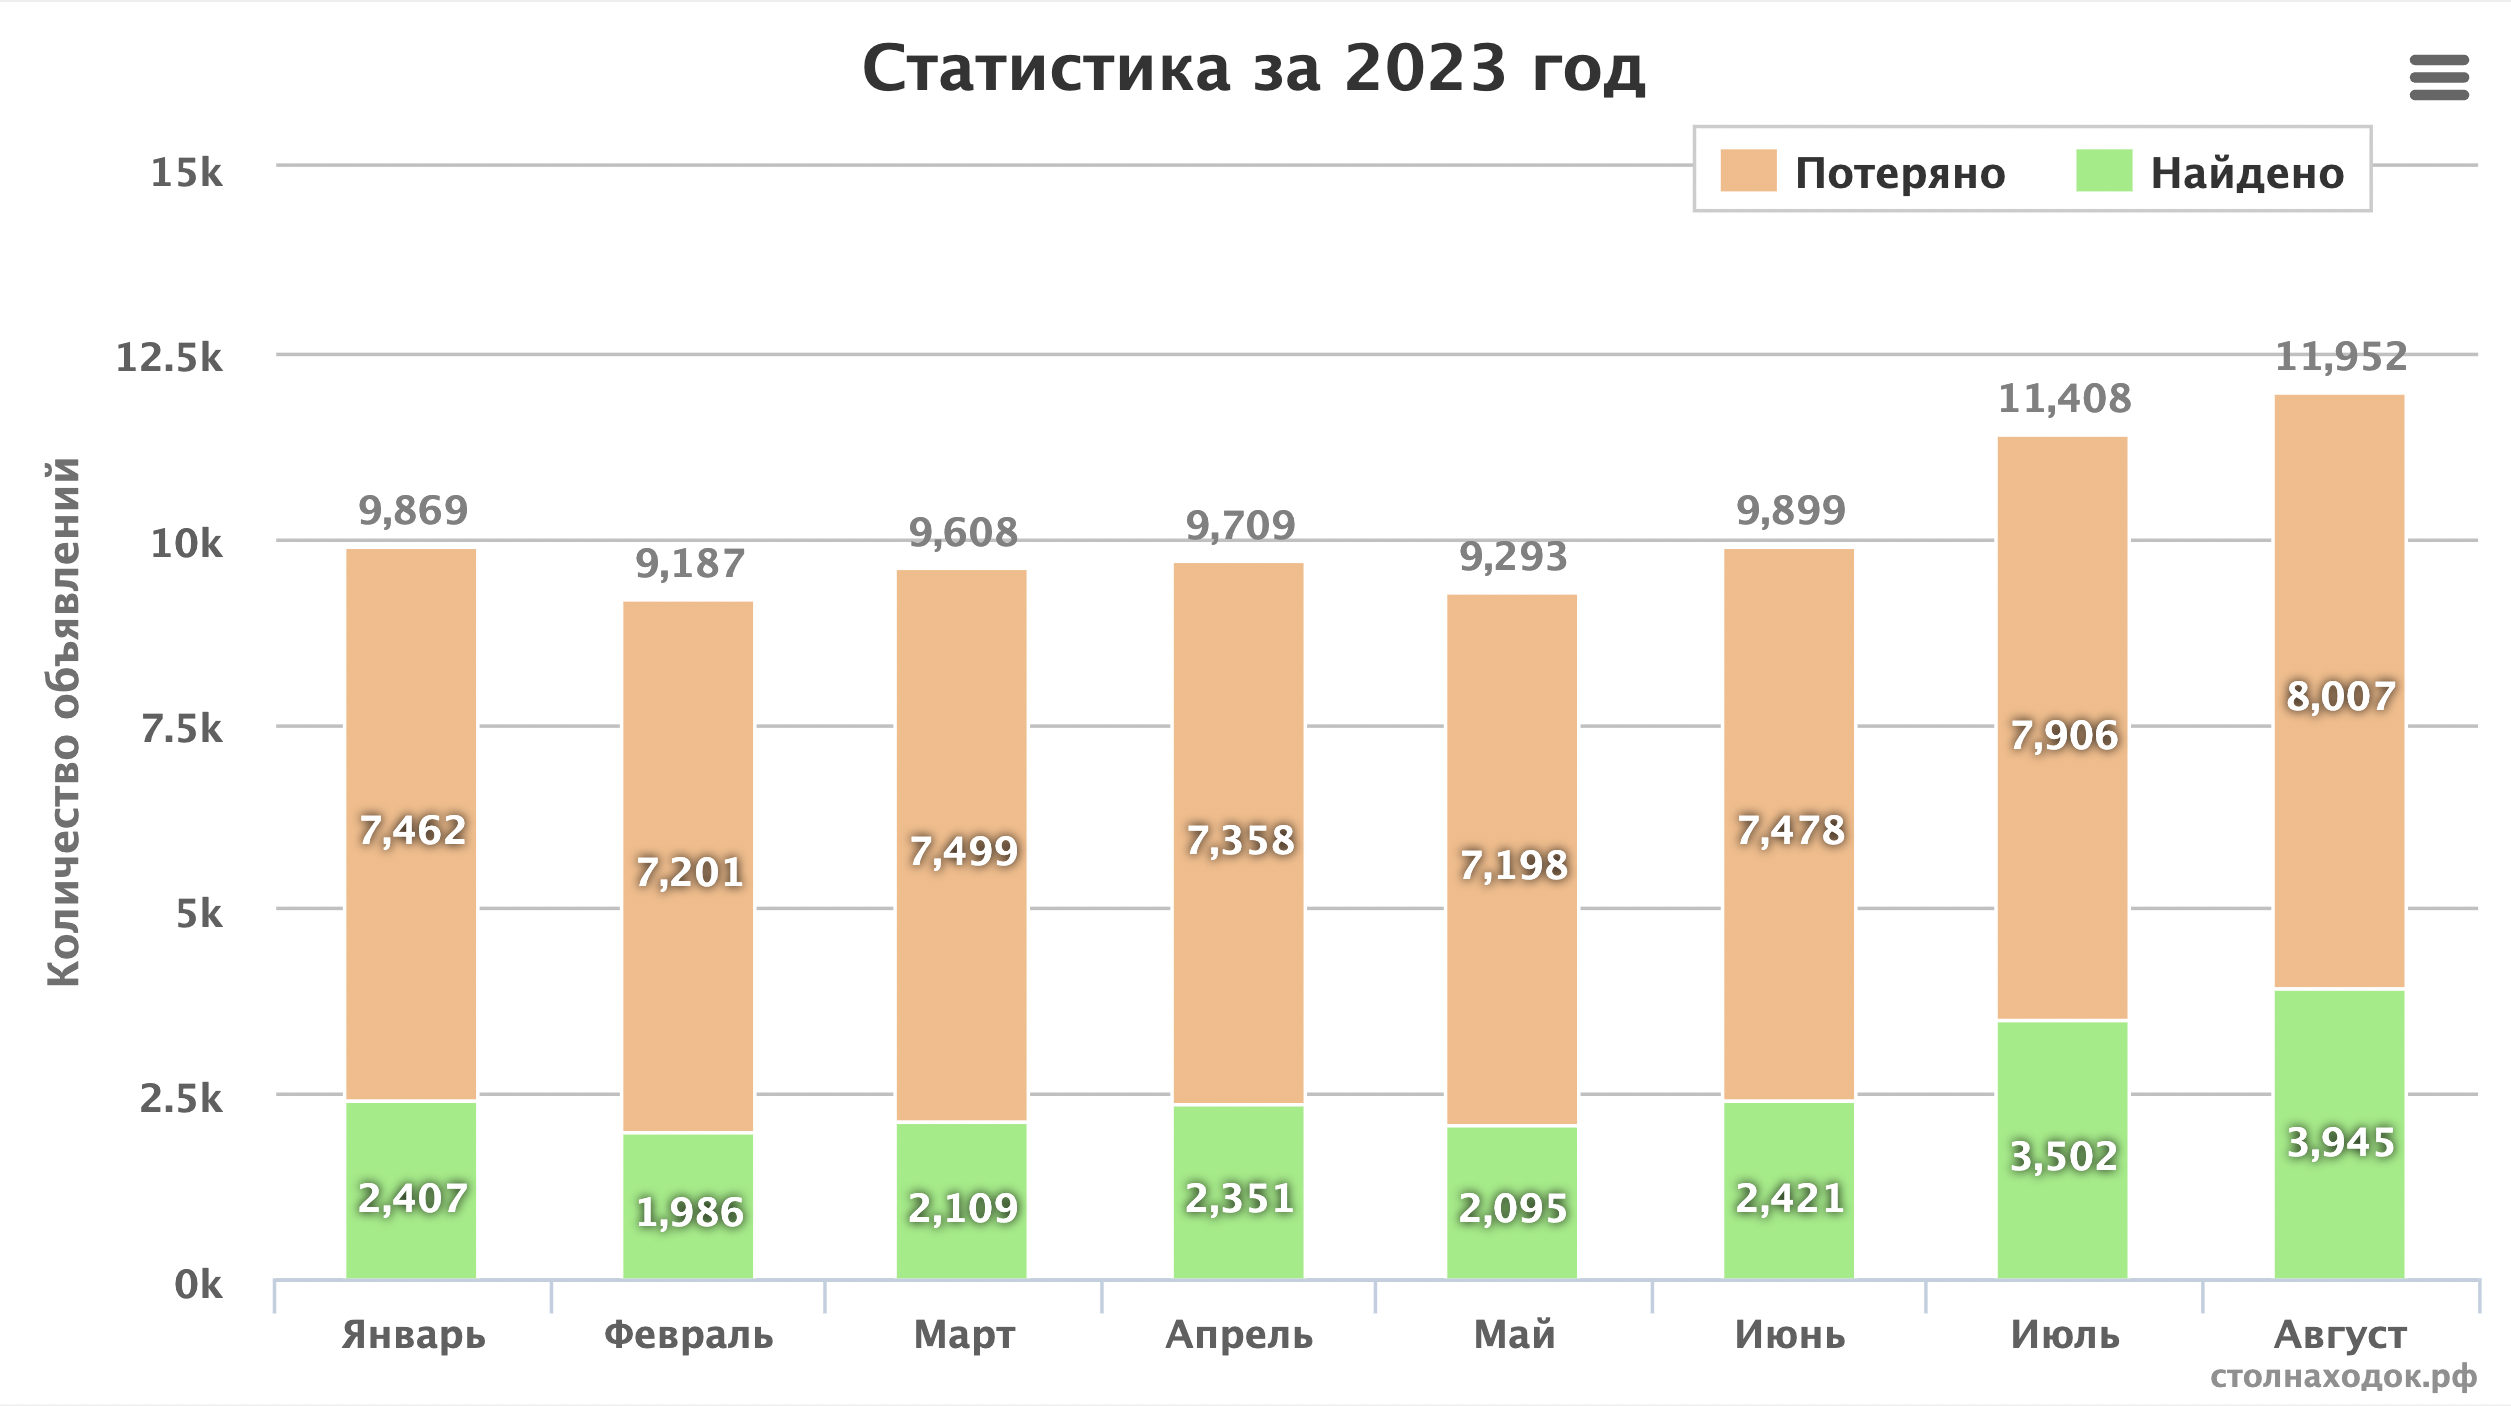
\includegraphics[width=.95\textwidth]{images/chart2023}
	\parskip=6pt
	\caption{Востребованность системы столнаходок.рф в 2023 году}
	\label{fig:chart2023}
\end{figure}

\begin{figure}[htb]
	\centering
	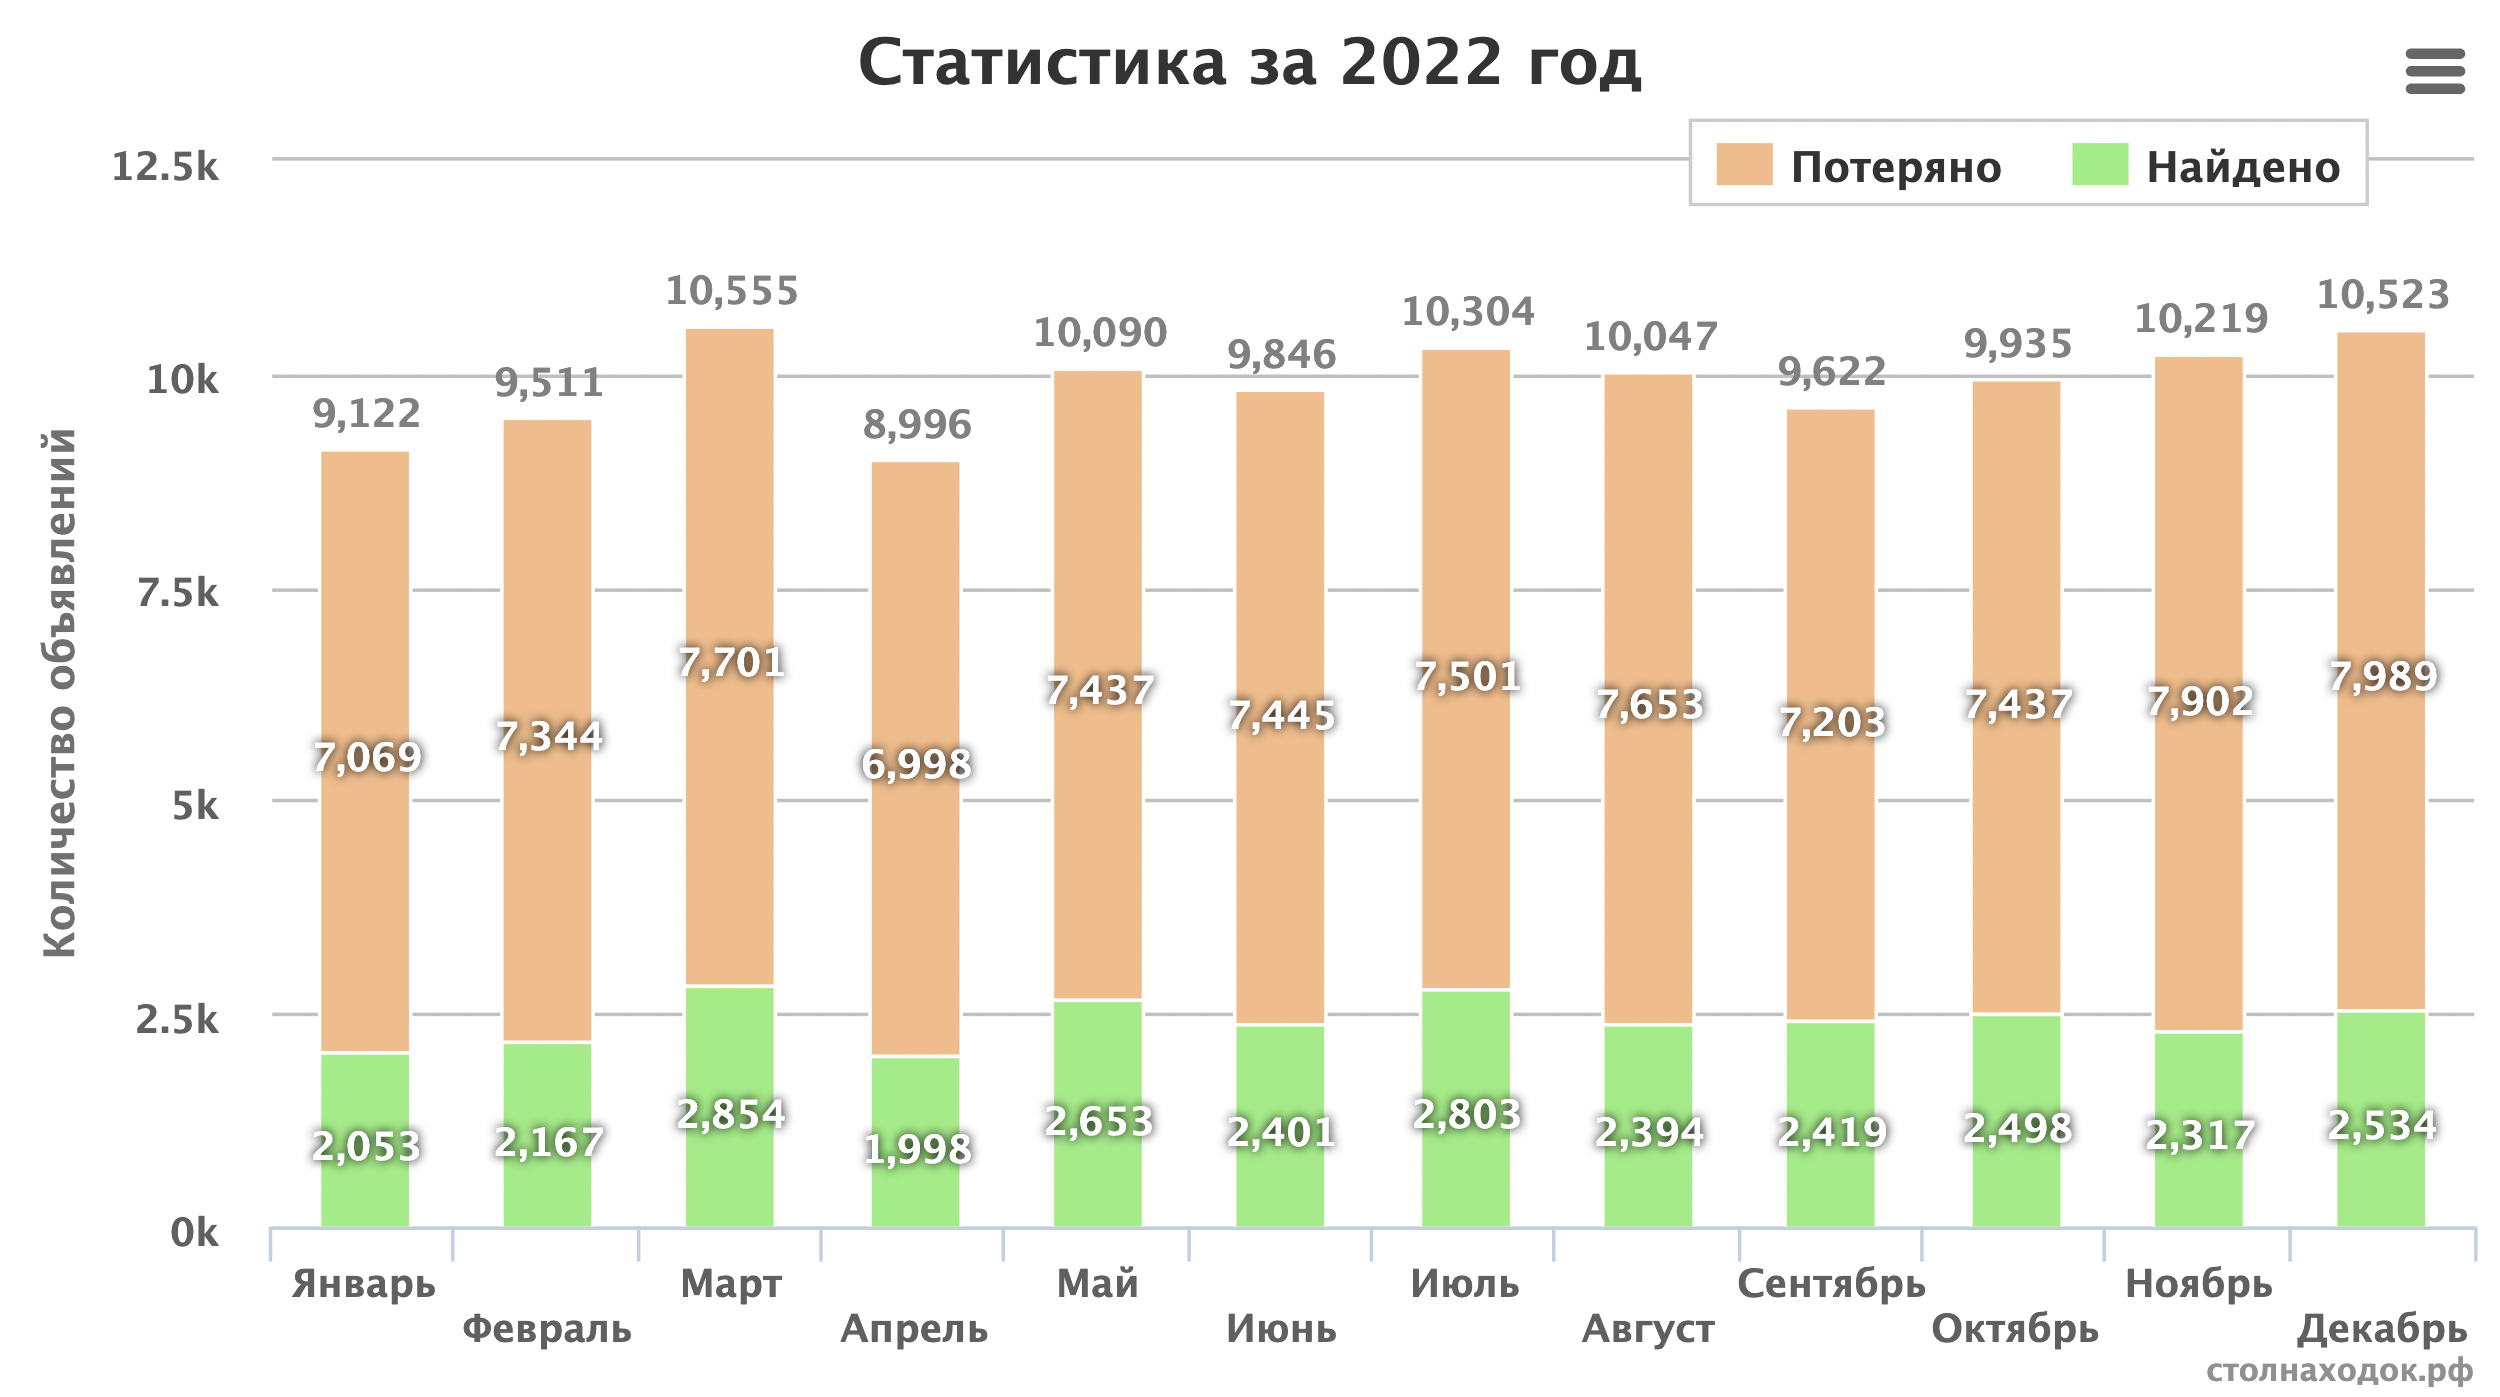
\includegraphics[width=.95\textwidth]{images/chart2022}
	\parskip=6pt
	\caption{Востребованность системы столнаходок.рф в 2022 году}
	\label{fig:chart2022}
\end{figure}

\subsection{Типы существующих решений для поиска и возврата утерянных вещей}

\begin{enumerate}
	\item[] Существует несколько типов существующих решений для поиска и возврата утерянных вещей. Ниже приведены некоторые из них:
	
	\item Веб-сайты и приложения "Бюро находок": Эти сервисы предоставляют платформу для регистрации утерянных вещей и поиска их владельцев. Пользователи могут создавать объявления о потерянных или найденных вещах и связываться друг с другом для возврата. Некоторые из этих сервисов предлагают возможность добавления фотографий или описания вещи для облегчения поиска.
	
	\item Технология RFID (Radio Frequency Identification): RFID-метки могут быть прикреплены к ценным вещам, и их сигнал может быть отслежен с помощью специального считывателя. Это позволяет пользователям быстро определить местоположение утерянных вещей через дополнительное программное обеспечение.
	
	\item GPS-трекеры: Эти устройства с GPS-модулем могут быть прикреплены к вещам, и их местоположение может быть отслежено с помощью специализированного приложения для смартфонов или веб-панели управления. Пользователи могут получать уведомления о перемещении вещи и быстро определить ее местонахождение.
	
	\item Автоматизированные системы обнаружения: Некоторые организации, такие как аэропорты или железнодорожные станции, имеют системы обнаружения утерянных вещей. Эти системы используют технологии, такие как видеонаблюдение, датчики движения или распознавание образов, чтобы отслеживать и возвращать потерянные вещи своим владельцам.
\end{enumerate}

Каждый из этих типов решений имеет свои преимущества и недостатки. Некоторые из них могут быть более подходящими для конкретных ситуаций, например, GPS-трекеры могут быть полезными при поиске утерянных вещей на открытой местности, в то время как RFID-метки могут быть более подходящими для использования внутри помещений. Веб-сайты и приложения <<Бюро находок>> предоставляют более универсальное решение, которое может быть использовано в различных ситуациях.

\subsection{Обзор существующих веб-сервисов и приложений для поиска и возврата утерянных вещей}

В настоящем разделе будет проведен обзор существующих веб-сервисов и приложений, которые предлагают функциональность поиска и возврата утерянных вещей. Данный обзор позволит выявить основные преимущества и недостатки этих сервисов, а также определить потенциальные возможности для улучшения их функциональности.

<<столнаходок.рф>>~\cite{bib:stol_nahodok} --- это один из наиболее популярных веб-сервисов, предоставляющих возможность объявлять о потерянных и найденных предметах. Сервис имеет простой и интуитивно понятный интерфейс, позволяющий пользователям быстро разместить информацию о потерянных вещах и связаться с владельцами найденных предметов. Однако, отсутствие системыуведомлений и неэффективное сопоставление объявлений ограничивают его функциональность.

<<Find My Stuff>>~\cite{bib:find_my_stuff} --- это мобильное приложение, разработанное для операционных систем iOS и Android. Оно предлагает функцию отслеживания утерянных предметов через GPS-модуль смартфона. Пользователи могут отмечать свои вещи на карте и получать уведомления, когда они находятся рядом с утерянным предметом. Однако, ограничение использования только наличием смартфона с GPS-модулем и низкая точность определения местоположения представляют существенные ограничения данного приложения.

<<Lost Property Office>>~\cite{bib:parliament_lost_and_found} --- это веб-сервис, предоставляемый государственными организациями и органами правопорядка. Сервис позволяет пользователям сообщать о потерянных и найденных предметах, а также предоставляет информацию о процедуре возврата утерянных вещей. Однако, ограниченный доступ к сервису и неудобный процесс регистрации и подачи заявки являются значительными недостатками данного сервиса.

На основании проведенного обзора можно сделать вывод, что существующие веб-сервисы и приложения для поиска и возврата утерянных вещей имеют некоторые преимущества, но также недостатки, которые ограничивают их функциональность и удобство использования. Веб-сервис Бюро находок будет разработан с учетом этих недостатков и предлагать более эффективное и удобное взаимодействие между пользователями и сервисом.

Ниже приведена сравнительная таблица~\ref{tab:analogs_comparison} основных характеристик и функций приведенных выше аналогов:
\begin{table}[htb]
	\caption{сравнительная таблица аналогов}
	\centering
	\begin{tabular}{ |p{2cm}|p{3cm}|p{2cm}|p{2cm}|p{3cm}|p{2cm}| } 
		\hline
		Сервис / Приложение & Интерфейс и удобство использования & Опове\-ще\-ния & Точность определения местоположения & Регистрация и подача заявки & Доступ\-ность \\ \hline
		
		Lost and Found & Простой и интуитивно понятный интерфейс & Отсут\-ству\-ют & Не\-оп\-ре\-де\-ле\-но & Простой процесс регистрации & Широкий доступ \\ \hline
		
		Find My Stuff & Простой и интуитивно понятный интерфейс & Опо\-ве\-ще\-ния через уведомления & Низкая точность & Простой процесс регистрации & Доступен только на смартфонах с GPS \\ \hline
		
		Lost Property Office & Неудобный процесс регистрации и подачи заявки & Отсут\-ству\-ют & Не\-оп\-ре\-де\-ле\-но & Неудобный процесс регистрации и подачи заявки & Огра\-ни\-чен\-ный доступ \\ \hline
	\end{tabular}
	\label{tab:analogs_comparison}
\end{table}

\subsection*{Вывод по разделу}

В аналитическом разделе моего исследования проведен подробный обзор различных существующих веб-сервисов и приложений, которые предназначены для поиска и возврата утерянных вещей. Мы изучили и проанализировали их функциональность, особенности, преимущества и недостатки.

Веб-сервисы и приложения <<Бюро находок>> представляют собой одно из самых популярных и широко используемых решений в данной области. Они предоставляют платформу, на которой пользователи могут зарегистрировать утерянные вещи и связаться с их владельцами. Это позволяет упростить процесс поиска и возврата утерянных вещей, обеспечивая удобный и интуитивно понятный интерфейс для пользователей.

Однако, помимо <<Бюро находок>>, существуют и другие типы решений. Например, RFID-метки, которые позволяют отслеживать сигнал утерянных вещей с помощью специального считывателя. Также существуют GPS-трекеры, которые оснащены GPS-модулем и позволяют отслеживать местоположение вещей с помощью приложений для смартфонов или веб-панелей управления.

Кроме того, существуют и автоматизированные системы обнаружения, которые используют различные технологии, такие как видеонаблюдение или распознавание образов, для отслеживания и возврата утерянных вещей. Эти системы могут быть полезны в ситуациях, где утерянные вещи могут быть обнаружены на основе визуальной информации или других характеристик.

Каждый из этих типов решений имеет свои преимущества и недостатки, и их эффективность может зависеть от конкретной ситуации. Веб-сервисы и приложения <<Бюро находок>> предоставляют наиболее универсальное решение, позволяющее пользователям зарегистрировать и найти утерянные вещи в различных ситуациях. Они предоставляют простой и интуитивно понятный интерфейс, а также систему уведомлений для повышения эффективности поиска.

\section{Специальный раздел}

\subsection{Требования к разрабатываемой системе}

TODO

\subsection{Проектирование архитектуры}

TODO

\subsection{Механизм поиска и сопоставления объявлений}

TODO

\subsection{Механизм обратной связи и взаимодействия пользователей}

TODO

\subsection{Меры безопасности и конфиденциальности}

TODO

\begin{comment}
\subsection{Монетизация и бизнес-модель}
\subsection{Планы по развитию и масштабированию}
\end{comment}

\subsection*{Вывод по разделу}

TODO

\section{Технологический раздел}

\subsection{Архитектура системы}

TODO

\subsection{Технические требования}

TODO

\subsection{База данных}

TODO

\subsection{Безопасность}

TODO

\subsection{Интерфейс пользователя}

TODO

\subsection*{Вывод по разделу}

TODO


\begin{comment}
\section{Экономический раздел}
\subsection{Планирование разработки программного продукта}
\subsection{Составление сметы затрат на разработку}
\subsubsection{Материальные затраты}
\subsubsection{Затраты на оплату труда}
\subsubsection{Амортизационные отчисления}
\subsubsection{Прочие расходы}
\end{comment}

\supersection{Заключение}

TODO



\begin{thebibliography}{99\kern\bibindent}
	\bibitem{bib:stol_nahodok} Бюро находок // столнаходок.рф: информационно-поисковый портал РФ URL: \url{http://nahodok.ru/} (дата обращения: 01.09.2023).
	\bibitem{bib:find_my_stuff} Find my stuff // fstuff.com: мобильное приложение URL: \url{https://www.fstuff.com/} (дата обращения: 01.09.2023).
	\bibitem{bib:parliament_lost_and_found} Lost Property Office // parliament.uk: веб приложение URL: \url{https://www.parliament.uk/visiting/access/facilities/lost-property/} (дата обращения: 01.09.2023).
\end{thebibliography}



\appendix

\section{Схема базы данных}

\begin{comment}
\begin{lstlisting}[label=lst:factorial]
model Account {
	id                String  @id @default(cuid())
	userId            String
	type              String
	provider          String
	providerAccountId String
	refresh_token     String?
	access_token      String?
	expires_at        Int?
	token_type        String?
	scope             String?
	id_token          String?
	session_state     String?
	user              User    @relation(fields: [userId], references: [id], onDelete: Cascade)
	
	@@unique([provider, providerAccountId])
}

model Session {
	id           String   @id @default(cuid())
	sessionToken String   @unique
	userId       String
	expires      DateTime
	user         User     @relation(fields: [userId], references: [id], onDelete: Cascade)
	
	@@index([userId], type: Hash)
}

model User {
	id                String              @id @default(cuid())
	name              String?
	nickname          String              @unique
	socialNetworks    UserSocialNetwork[]
	email             String?             @unique
	emailVerified     DateTime?
	userInfo          String?             @db.VarChar(280)
	role              Role                @default(USER)
	image             String?
	isBlocked         Boolean             @default(false)
	blockReason       String?
	accounts          Account[]
	sessions          Session[]
	lostAndFoundItems LostAndFoundItem[]
	
	@@index([id], type: Hash)
	@@index([nickname], type: Hash)
}

model VerificationToken {
	identifier String
	token      String   @unique
	expires    DateTime
	
	@@unique([identifier, token])
}

model UserSocialNetwork {
	id                             String                           @id @default(cuid())
	socialNetwork                  SocialNetwork
	link                           String
	userId                         String
	user                           User                             @relation(fields: [userId], references: [id], onDelete: Cascade)
	lostAndFoundItemSocialNetworks LostAndFoundItemSocialNetworks[]
	
	@@unique([userId, socialNetwork])
	@@index([socialNetwork, userId])
}

enum Role {
	USER
	MODERATOR
	ADMIN
}

model LostAndFoundItem {
	id             String                           @id @default(cuid())
	name           String                           @db.VarChar(100)
	description    String                           @default("") @db.VarChar(512)
	campus         Campus
	reason         PostItemReason
	status         LostAndFoundItemStatus           @default(ACTIVE)
	images         String[]
	userId         String
	user           User                             @relation(fields: [userId], references: [id], onDelete: Cascade)
	socialNetworks LostAndFoundItemSocialNetworks[]
	created        DateTime                         @default(now())
	expires        DateTime                         @default(dbgenerated("NOW() + interval '1 week'"))
	
	@@index([id], type: Hash)
}

enum LostAndFoundItemStatus {
	ACTIVE
	EXPIRED
	BLOCKED
}

model LostAndFoundItemSocialNetworks {
	id                  String            @id @default(cuid())
	lostAndFoundItemId  String
	lostAndFoundItem    LostAndFoundItem  @relation(fields: [lostAndFoundItemId], references: [id], onDelete: Cascade)
	userSocialNetworkId String
	userSocialNetwork   UserSocialNetwork @relation(fields: [userSocialNetworkId], references: [id], onDelete: Cascade)
	
	@@unique([lostAndFoundItemId, userSocialNetworkId])
}

enum PostItemReason {
	LOST
	FOUND
}

enum Campus {
	V78
	S20
	V86
	MP1
	SG22
	SHP23
	U7
}

enum SocialNetwork {
	TELEGRAM
	VK
}
\end{lstlisting}
\end{comment}

	
\end{document}